\documentclass[letterpaper,conference]{IEEEtran}
%% CCNC 2013 addition:
%\makeatletter
%\def\ps@headings{%
%	\def\@oddhead{\mbox{}\scriptsize\rightmark \hfil \thepage}%
%	\def\@evenhead{\scriptsize\thepage \hfil \leftmark\mbox{}}%
%	\def\@oddfoot{}%
%	\def\@evenfoot{}}
%\makeatother
%\pagestyle{headings}

\setlength{\textheight}{9.21in}

\ifCLASSINFOpdf
	\usepackage[pdftex]{graphicx}
	\usepackage{epstopdf}
	\graphicspath{{./figures/}}
	\DeclareGraphicsExtensions{.pdf,.jpeg,.jpg,.png,.eps}
\else
	\usepackage[dvips]{graphicx}
	\graphicspath{{./figures/}}
	\DeclareGraphicsExtensions{.eps}
\fi

\usepackage[cmex10]{amsmath}
\interdisplaylinepenalty=2500
\usepackage{dblfloatfix}
\usepackage{url}

%\IEEEoverridecommandlockouts

% Title Page
\title{Byte-By-Night: Web Cache Object Forwarding from Desktop to Mobile for Energy Consumption Optimizations}
\author{
\IEEEauthorblockN{Troy Johnson}
\IEEEauthorblockA{Department of Computer Science\\
	Central Michigan University\\
	Mount Pleasant, MI 48859\\
	johns4ta@cmich.edu
}
\and
\IEEEauthorblockN{Patrick Seeling\thanks{Please direct correspondence to P. Seeling}}
\IEEEauthorblockA{Department of Computer Science\\
	Central Michigan University\\
	Mount Pleasant, MI 48859\\
	pseeling@ieee.org\footnote{Please direct correspondence to P. Seeling.}}
}

\begin{document}
\maketitle
\pagestyle{empty}
\thispagestyle{empty}
\begin{abstract}
	\boldmath

\end{abstract}

\begin{IEEEkeywords}
%	Mobile applications, Android, connectivity, network traffic
Mobile communication; Middleware; Energy consumption
\end{IEEEkeywords}

\section{Introduction}
With the beginning of the 21st century, new support for mobile connected user devices has fueled a continuous increase in the demand for mobile data.
Web requests now originate in a majority from wirelessly connected user devices, a trend that is likely to continue in the foreseeable future~\cite{ciscovni}.
Simultaneously, the overall user behavior and demand for more rich media inclusion into web pages has increased the overall amount of data that is required to be transmitted per page, see, e.g., \cite{}.
Caching on the client side has been effectively used in the past and was, together with increased numbers of parallel object downloads, able to decrease wait times for desktop clients as reported in \cite{.}.


The remainder of this paper is structured as follows.
In the following section, we describe our overall scenario before we provide an example based on a particular web page.
In the subsequent Section~\ref{s:large}, we discuss the overall properties of a large web page dataset archive and provide a simulation-driven evaluation of our approach.
We conclude in Section~\ref{s:conc}.


\section{Scenario Description }

\begin{figure}
	\centering
	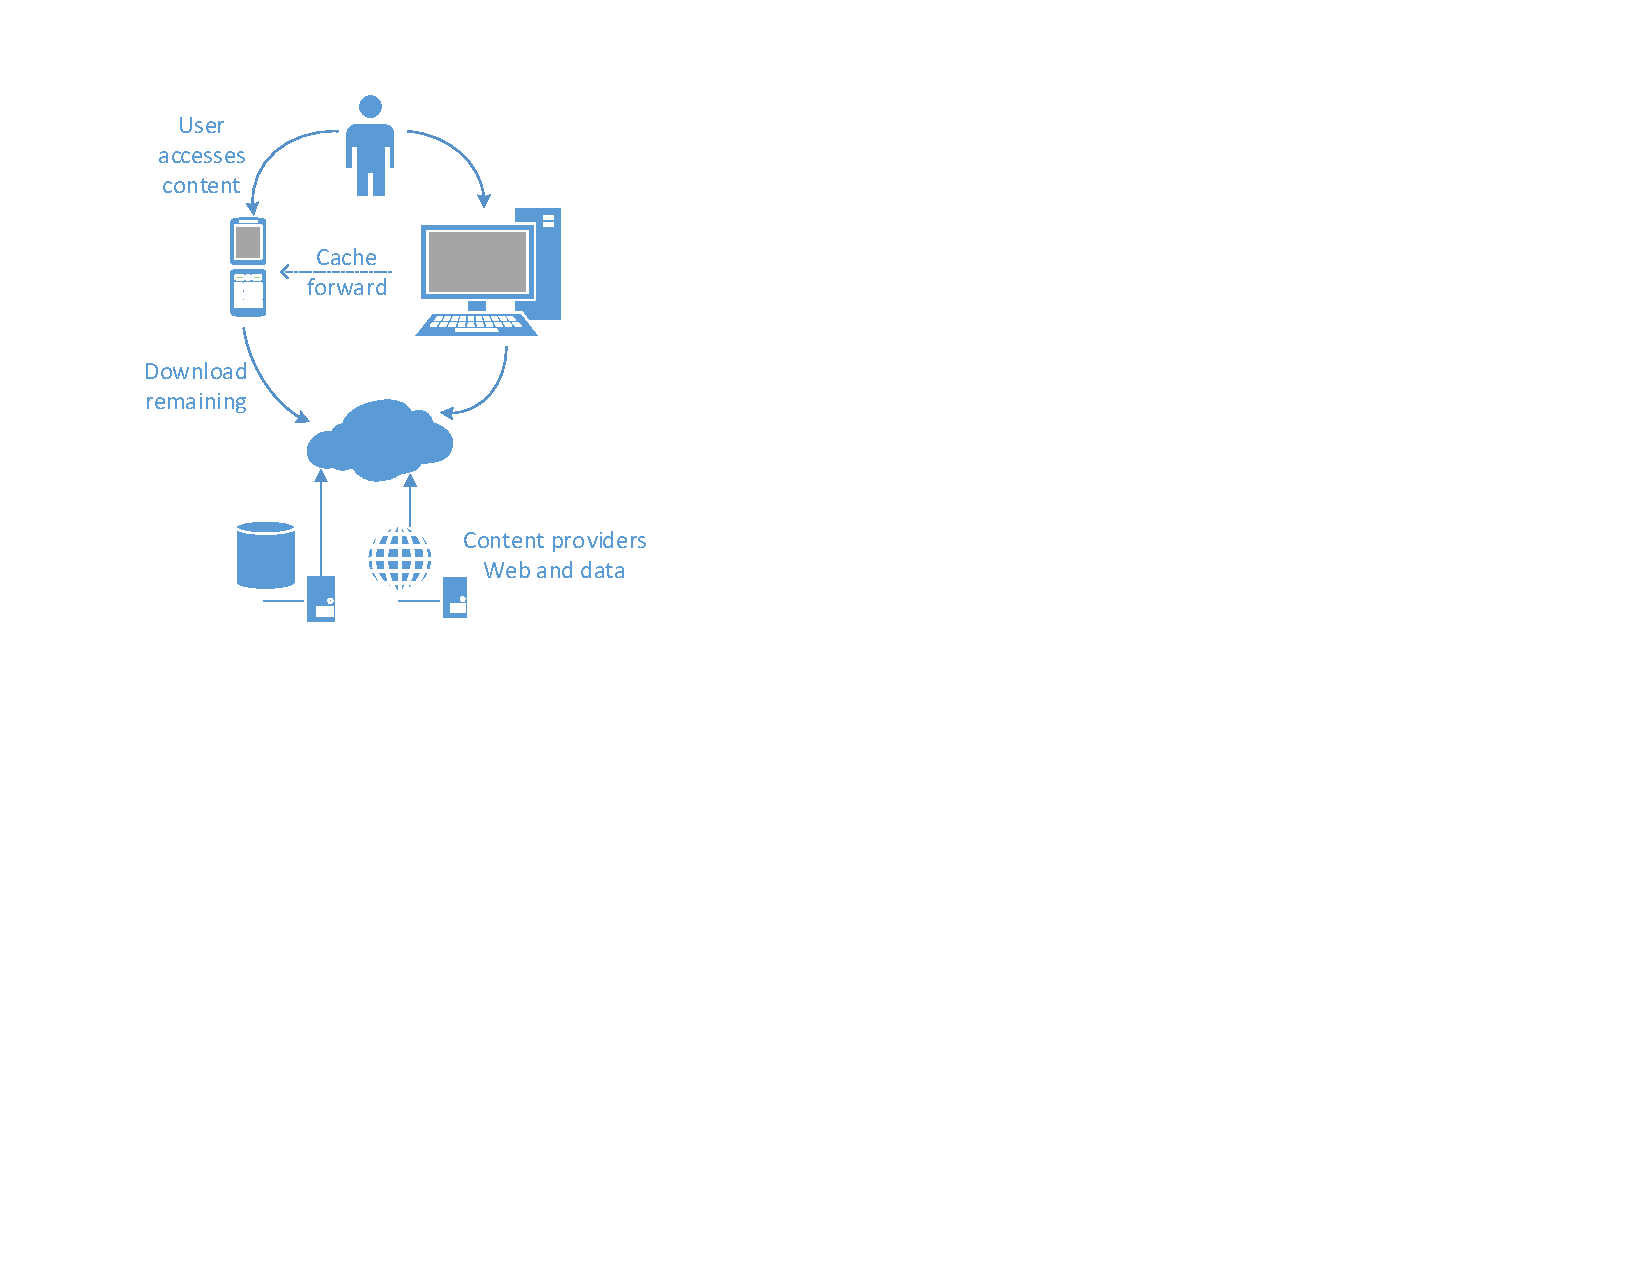
\includegraphics[width=.9\linewidth]{Drawing1}
	\caption{Overall setup of world wide web based content access by a user over time using primary and secondary devices to display the same content. If the devices are able to synchronize their caches through short-range communications, energy savings become possible.}
	\label{fig:setup}
\end{figure}



\section{Individual Example}
In this section, we outline an individual example for the German news web page for ``Der Spiegel,'' accessible at \url{http://www.spiegel.de} as an example for a rich media and advertising material containing web presence that is frequently updated.
On [insert final date], we performed a speed test online using Internet Explorer as browser instance for a desktop client, Chrome as mobile browser on a Google Nexus 5 instance, and Safari for an iPhone 4 instance provided by \url{WebpageSpeedTest.org} (both mobile clients were traffic shaped to 3G connection emulations).
An example screenshot of the web page as rendered is provided in Figure~\ref{fig:screens}.
\begin{figure}
	\centering
	
\includegraphics[width=.9\linewidth]{1screen}
	\caption{Screenshot of rendered webpage from WebPageSpeedTest.org. As illustrated, the main textual and pictorial content items are flanked by background and interactive advertisements.}
	\label{fig:screens}
\end{figure}

\subsection{Metrics}
We evaluate the reported data as follows. For each display modality, we gather the individual web objects requested and the response sizes and headers for caching information (for HTTP response codes 200 only, as we are not interested in redirects).
We denote the number of all objects returned for a request modality (i.e., Internet Explorer for the desktop client example and iPhone or Nexus 5 for mobile counterparts) as $N$, their average size as $\overline{X}$, the standard deviation of their sizes as ${\sigma}_{X}$, and the Coefficient of Variation (CoV) of the returned object sizes as $\mathrm{CoV}_{X}$. As in the HTTP specification, the \emph{max-age} directive overrides others, so we initially consider that directive for the cache longevity of the individual objects. If no explicit information is found, we consider the header's \emph{expires} information, which provides a secondary cache lifetime. If both are not found, or if the \emph{expires} date is in the past or right at the request time, we set the cache lifetime we consider here to zero. 
Similar to the notation for the object sizes, we denote the expiration time characteristics as $\overline{T}$, $\sigma_{T}$, and $\mathrm{CoV}_{T}$, respectively.
In case of size differences between the three, we utilize the smallest size as lower boundary.


\subsection{Data Description}

We provide an initial high-level overview of the webpage characteristics for \url{http://www.spiegel.de} as requested in Table~\ref{tab:spiegel}.
\begin{table}
\centering
\caption{High-level overview of different client webpage statistics for http://www.spiegel.de}
\label{tab:spiegel}
\begin{tabular}{|l|r|r|r|}
	\hline
	Statistic          & IE Deskt. &    iPhone &   Nexus 5 \\ \hline
	$N$                &       154 &       132 &       145 \\ \hline\hline
	$\overline{X}$     &  10402.77 &   8846.39 &  10201.63 \\ \hline
	$\sigma$           &  19103.19 &  13438.05 &  25684.58 \\ \hline
	$\mathrm{CoV}_{X}$ &      1.84 &      1.52 &      2.52 \\ \hline\hline
	$\overline{T}$     & 106285.14 & 114780.69 & 114818.28 \\ \hline
	$\sigma_{T}$       & 125080.27 & 125576.65 & 126090.90 \\ \hline
	$\mathrm{CoV}_{T}$ &      1.18 &      1.09 &      1.10 \\ \hline
\end{tabular}
\end{table}

We initially observe that the desktop version (with Internet Explorer 9 as requesting browser client) exhibits the highest number of objects, followed by the mobile Chrome/Android and Safari mobile/iOS versions, respectively. 
Interestingly, there is only a minor difference in the number of objects between these versions.
Next, we observe that the trend for the average number of bytes is aligned with the number of elements. 
In total, the mobile Chrome version is almost on par with the desktop one (at 92\%) and only the Safari mobile version seeming optimized (at 72\%).
The standard deviation and Coefficient of Variation (CoV) amongst individual element sizes are highest for the mobile Chrome version, indicating more significant size differences than for the safari version, which is one unit lower, while the desktop version falls into the middle.

Next, we evaluate the elements' caching properties on a high level in Table~\ref{tab:spiegel}. 
Overall, we note that the highest average caching time is observed for the mobile Chrome access with the Nexus 5 device, trailed immediately by the iOS access and with distance by the desktop browser.
We note that the overall variability in terms of expiration times amongst elements is fairly low and comparable, as indicated by CoV values around 1.1.

\subsection{Evaluation of Local Cache Synchronization}
We now shift the view to the possibility for identical objects to be re-utilized locally to avoid additional download penalties in time and energy consumption.
Simultaneous with a web page request, a local broadcast could ``ask'' for the cached elements for a website to be delivered locally form participating clients. Alternatively, cellular provisioning methods, such as in LTE-A, could initiate the device-to-device local exchange as well.
Once the request is received, the local coordination can take place, which inherently results in the forwarding of elements that are the same across browser instances and which have a future cache lifetime expiration.

We filter out elements that are not similar amongst the different requesting devices, which results in 82 objects with the same URL and size combination. 
While we note an identical cache lifetime for most of these, a slight increase is notable from the Desktop over Safari to Chrome.  Next, we remove items that exhibit a cache lifetime of zero for any of the three requesting clients, resulting in 59 objects, which now exhibit a reduced average cache lifetime for the mobile browsers, whereby mobile Chrome exhibits the shortest.
In turn, we choose the iOS Safari mobile as our exemplary base for calculations. 
We utilize the approximations for energy consumptions presented in~\cite{PeFiWi11} to determine the amount of energy required as time progresses if local data exchange can be performed using either Bluetooth or WLAN technologies. 
\begin{figure}
	\centering
	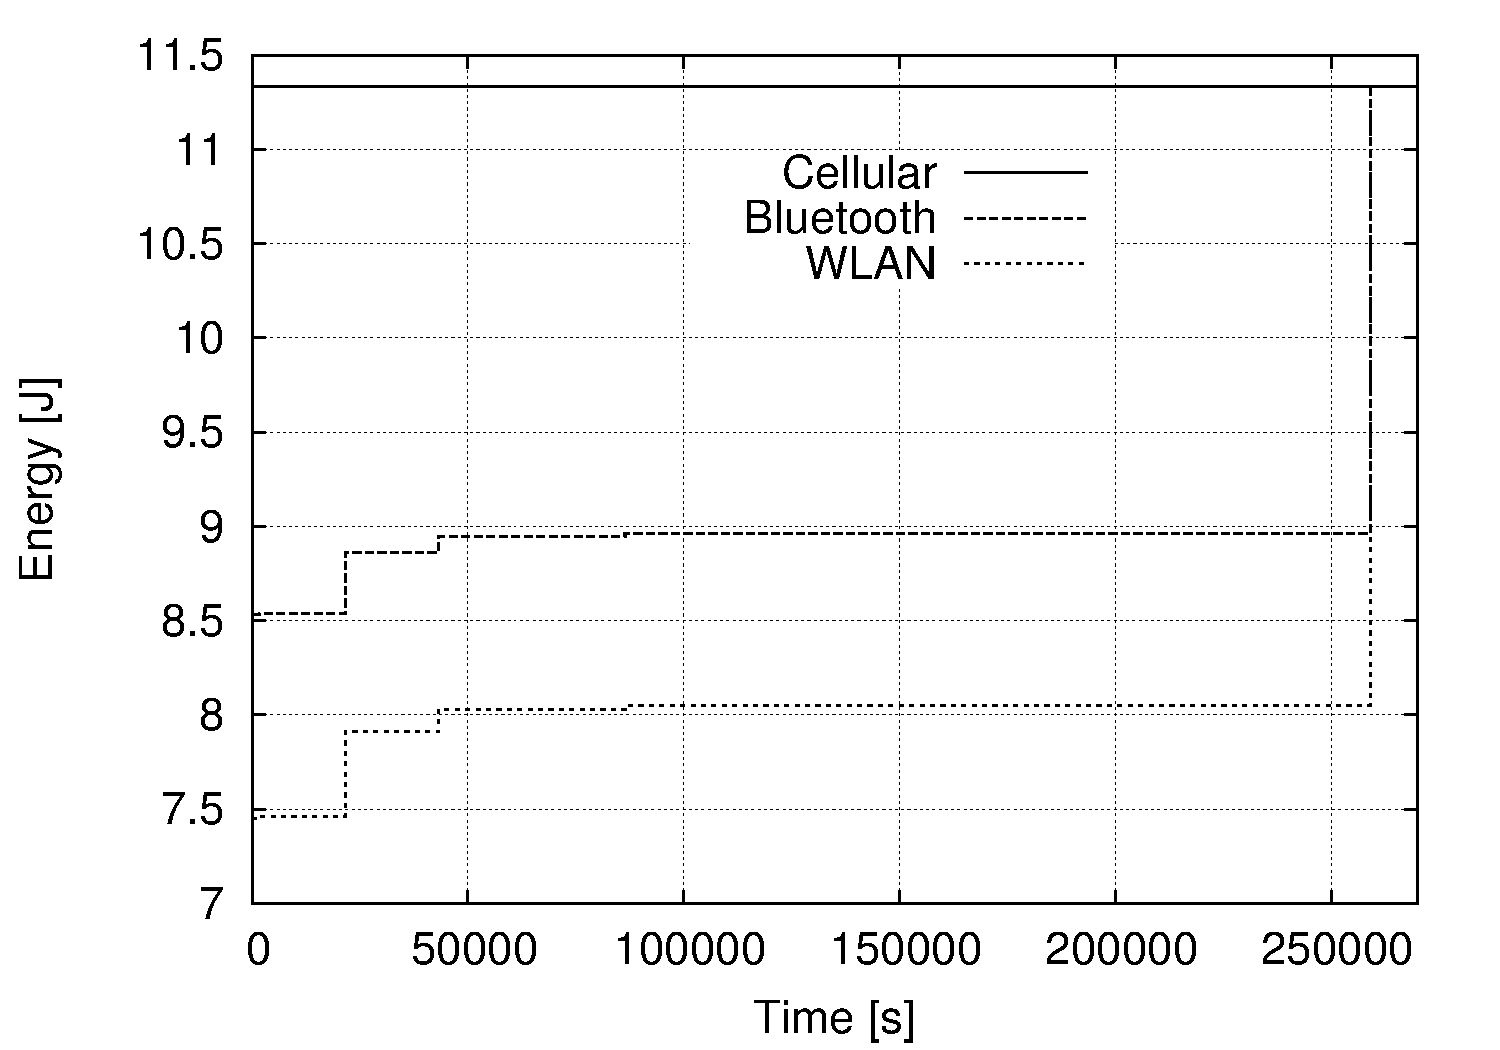
\includegraphics[width=.95\linewidth]{energy_ios_time}
	\caption{Energy required to download web page data via cellular connection or through combination with partial local exchange with Bluetooth/WLAN.}
	\label{fig:ios_time_energy}
\end{figure}
As illustrated, the complete download energy for cellular data is the upper limit on energy spent downloading the data associated with the web page. 
The Bluetooth and WLAN data exchanges with other local clients both follow the same underlying trend with increasing energy required to transmit all data as time progresses from the last access point in time.

We illustrate the relative amount of data/items within the cache in addition to the attainable savings in Figure~\ref{fig:rel_ios_time} as a function of delayed access time. 
\begin{figure}
	\centering
	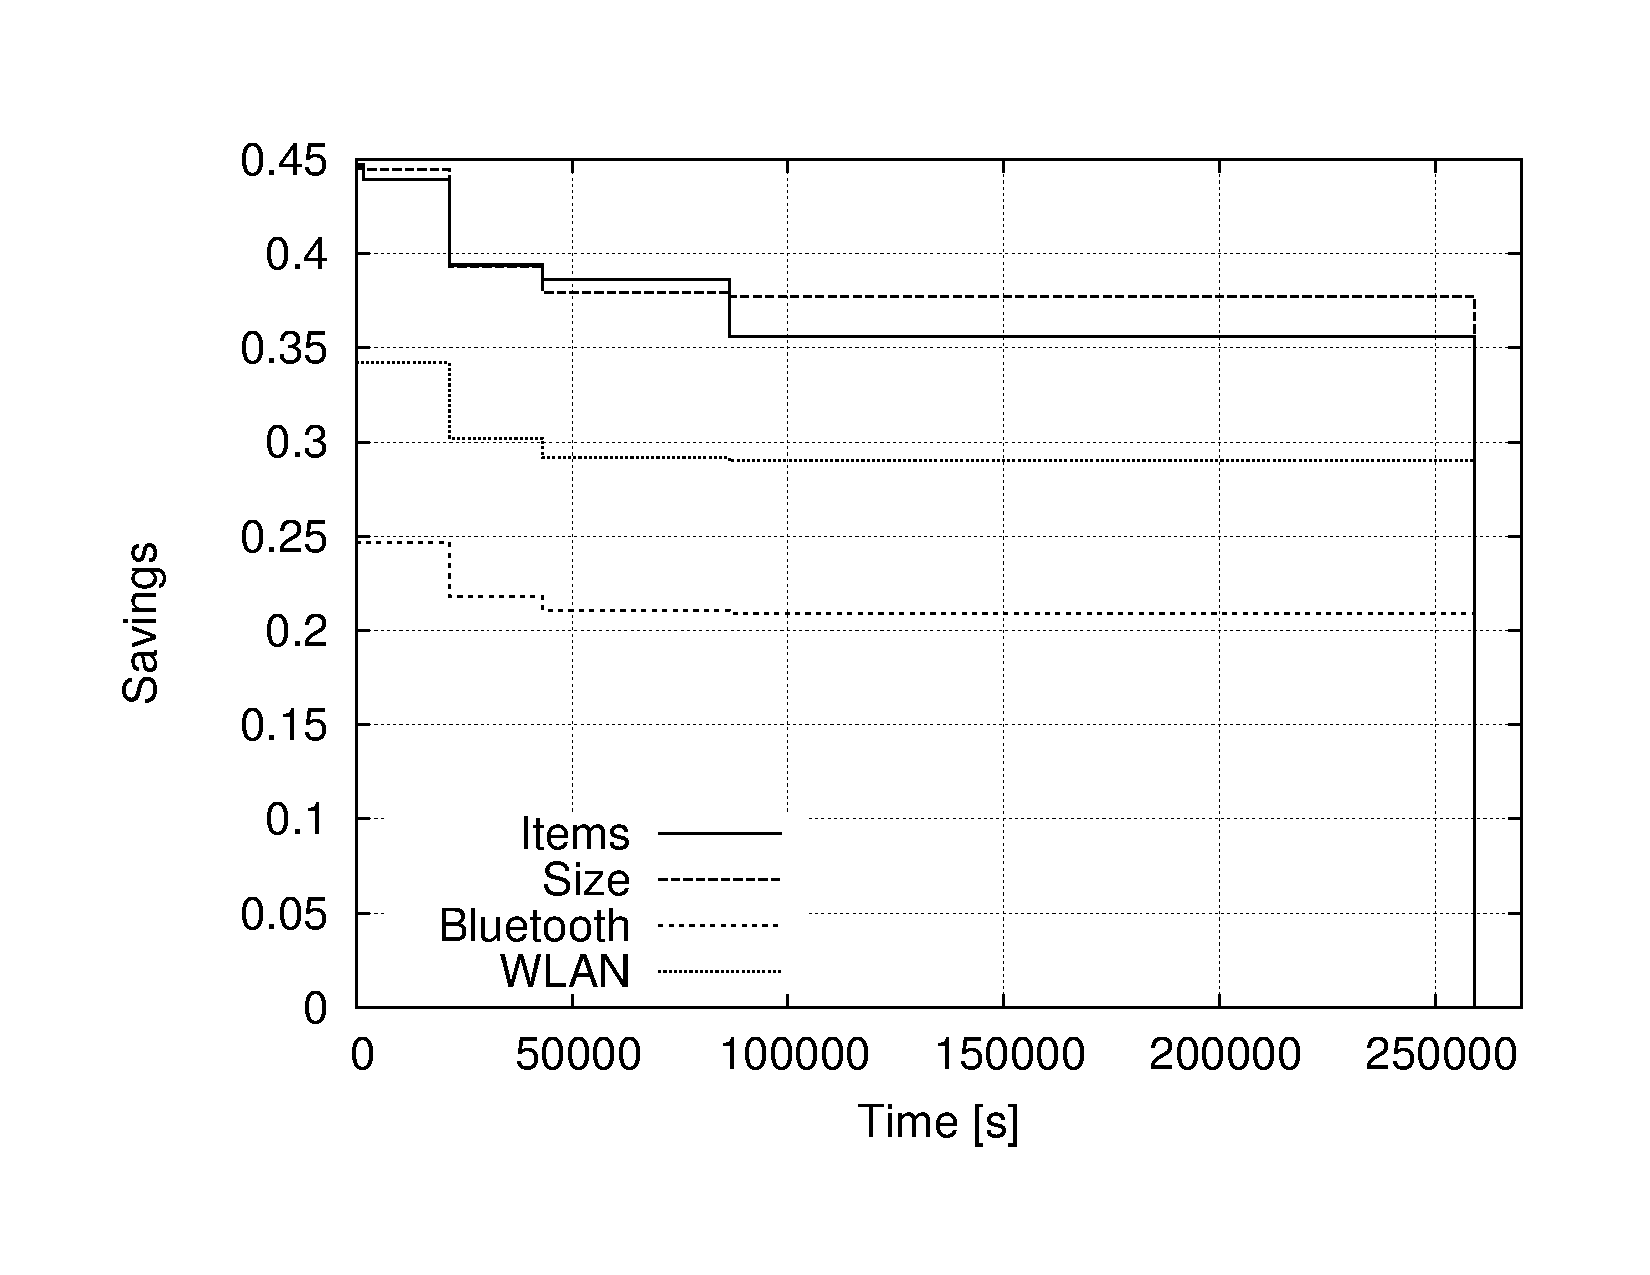
\includegraphics[width=.95\linewidth]{rel_ios_time}
	\caption{Relative number of items and data amounts in cache and savings resulting from local data exchange with }
	\label{fig:rel_ios_time}
\end{figure}
We observe that a significant amount of the overall data can be cached (and would in turn be suitable for localized sharing).We additionally observe that even for longer durations up to multiple days, significant amounts of data remain in the cache.
Combining the streaming from local clients through either Bluetooth or WLAN technologies, we utilize the approximations outlined in~\cite{} to derive the relative gains of our approach in terms of energy consumption. 
Specifically, we compare our approach (combining locally exchanged caches and cellular downloads of the remainder) with the regular download of all items through the cellular network interface. 


\section{Large Dataset Performance Evaluation}
\label{s:large}
We now evaluate our proposed approach through simulations based on a large dataset of landing web pages of the most popular websites.
For this purpose, we retrieved the publicly available web page response details from \emph{httparchive.org} and create a subsequent dataset for the October 1st, 2013 dataset.

\subsection{Dataset Description}
The dataset we utilize for the performance evaluation contains the individual web responses for the most popular websites of fixed (Internet Explorer for the desktop) and mobile (iOS for iPhone 4) websites, ranked through the Alexa popularity index.
Furthermore, the dataset contains the individual response details, including cache expiration times and sizes. 

Similar to the individual web page example, we provide an overall description of the response sizes and maximum expiration ages in Table~\ref{tab:dataset}.
\begin{table*}
\centering
\caption{.}
\label{tab:dataset}
\begin{tabular}{|l||c|c|c|c||c|c|c|c|}
	\hline
	Category                         & \multicolumn{4}{|c||}{Desktop (IE)}                       & \multicolumn{4}{|c|}{Mobile (iOS)}                      \\
	                                 & $\sum X_i $ &   $N$    & $\sigma(X_i)$ & $\overline{X_i}$ & $\sum X_i $ &  $N$   & $\sigma(X_i)$ & $\overline{X_i}$ \\
	                                 &    [MB]     &          &     [kB]      &       [kB]       &    [MB]     &        &     [kB]      &       [kB]       \\ \hline\hline
	expAge $<$ 30 Seconds            &  238490.28  & 15670679 &    1698.59    &      15.22       &   1355.24   & 122598 &    582.98     &      11.05       \\ \hline
	30 $\le$ expAge $<$ 1 Minute     &   170.94    &  29130   &     27.38     &       5.87       &    12.68    &  898   &     70.38     &      14.12       \\ \hline
	1 Minute $\le$ expAge $<$ 1 Hour &  15192.40   &  797450  &    270.06     &      19.05       &   282.36    & 15854  &    226.62     &      17.81       \\ \hline
	1 Hour $\le$ expAge $<$ 12 hours &  29798.68   & 1186947  &    751.45     &      25.11       &   244.14    & 17424  &    209.84     &      14.01       \\ \hline
	12 hours $\le$ expAge $<$ 1 day  &   6188.57   &  358998  &    227.63     &      17.24       &    91.37    &  5952  &     91.37     &      15.35       \\ \hline
	1 day $\le$ expAge               &  195784.64  & 9888147  &    1337.36    &      19.80       &   2122.96   & 126629 &    750.51     &      16.77       \\ \hline\hline
	Average                          &  80937.59   & 4655225  &    718.75     &      17.39       &   684.79    & 48226  &    321.95     &      14.20       \\ \hline
\end{tabular}
\end{table*}
We note that the overall average response size as result of desktop requests (when batched into the outlined time frames) is around of 17 kB, with the largest average sizes occurring between one and twelve hours.
Mostly, we note that the majority of objects exhibit a short expiration time between zero and 30 seconds.
For the responses to mobile devices, we note that the majority of objects are in the same short time span and the long time span of more than one day.
The highest average response sizes, however, are observed between one hour and half a day, in difference to the desktop counterpart.

We illustrate the cumulative distribution for the desktop and mobile client response expiration ages in Figure~\ref{fig:comp_cpd}.
\begin{figure}
	\centering
	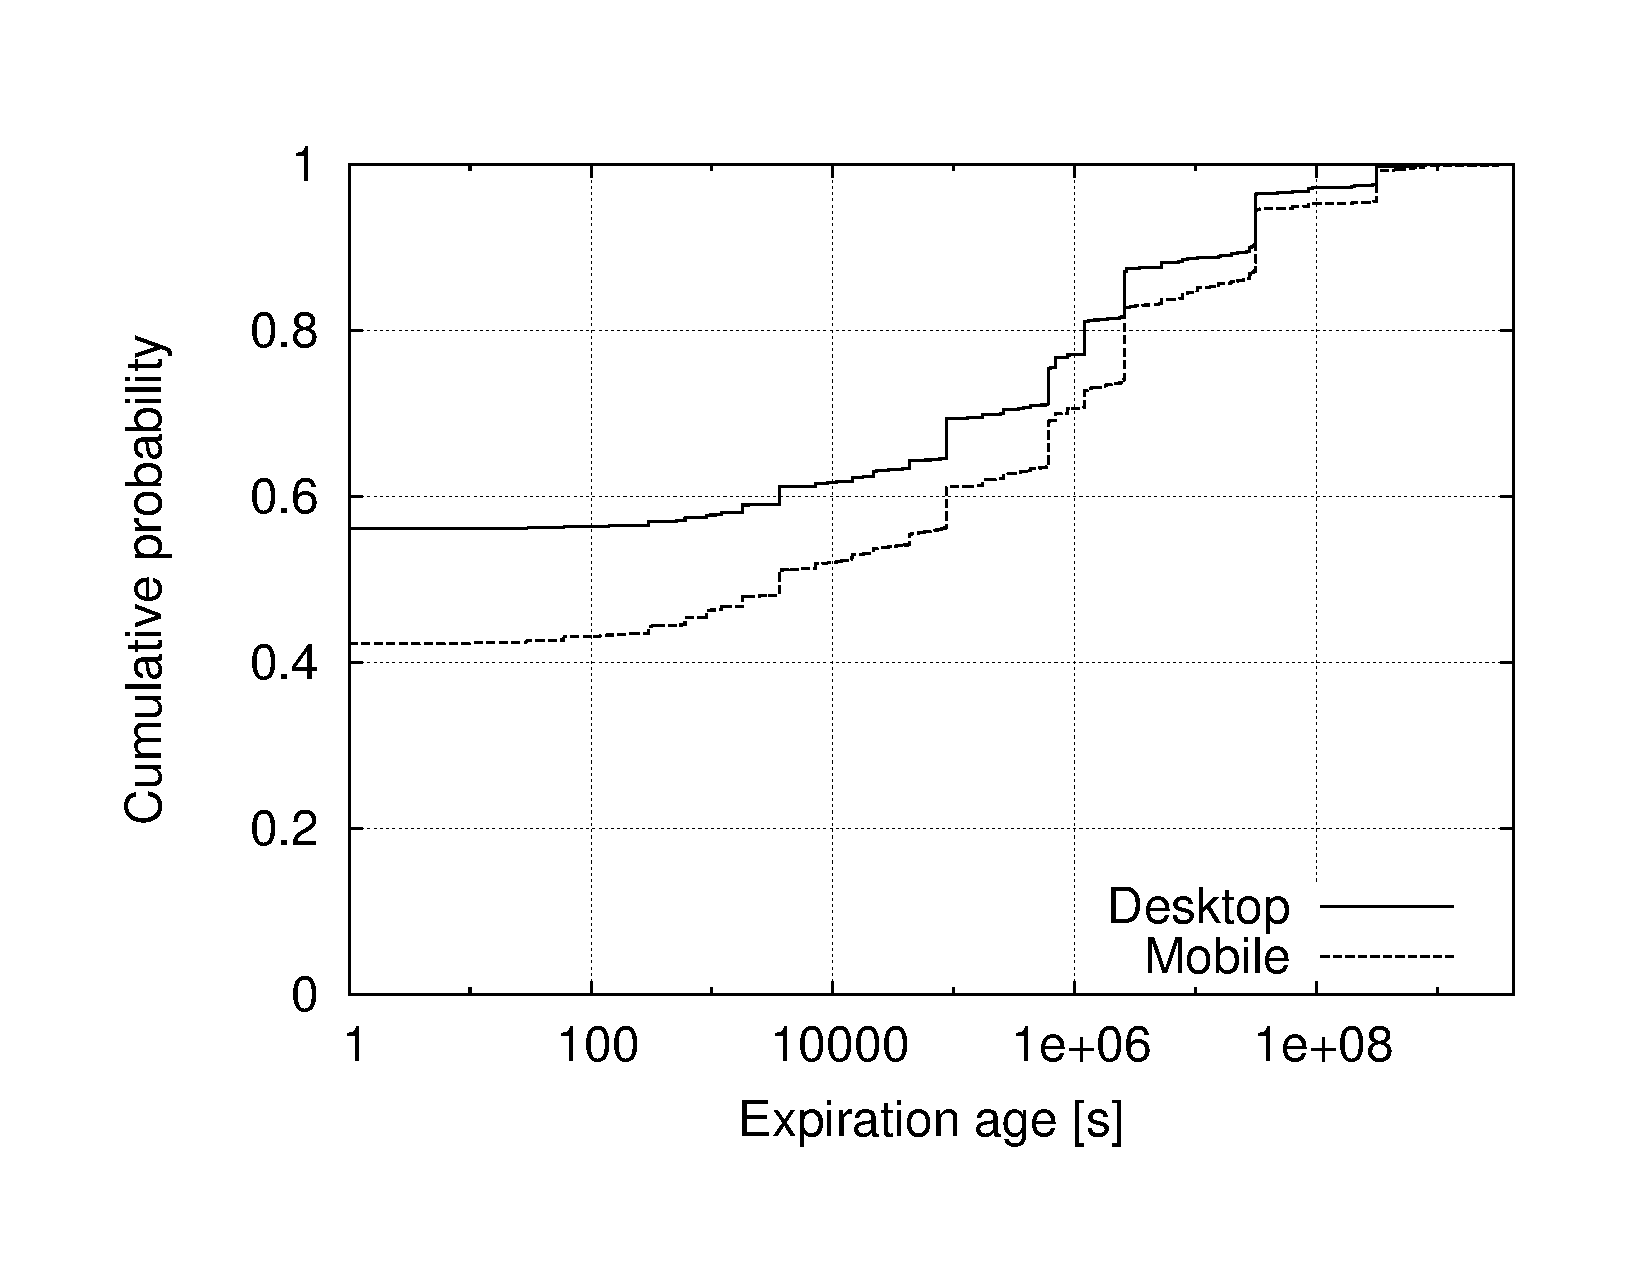
\includegraphics[width=.95\linewidth]{comp_cpd}
	\caption{Cumulative probability  }
	\label{fig:comp_cpd}
\end{figure}
We observe that a significant portion ($>40$ \%) of responses form web servers exhibits an immediate expiration and would, in turn, require an immediate retrieval by clients.
The cumulative expiration probability is higher for responses to desktop clients, which can be attributed to the typically more abundant bandwidth (and less optimization requirements) in contrast to a mobile setting (where web content developers might be more considerate of limitations).


\subsection{Simulation Model Description}
%\ref{we use the simple zipf distribution to make life easy?} 
We evaluate the effectiveness of our approach through simulation, which we perform as follows.
For the time period of one week, we randomly select a web page from the mobile dataset and separate the data that is required to be downloaded and the data that is still available in cache due to the maximum expiration age of the individual objects. We subsequently wait for a random amount of time before repeating the procedure.
We now describe the process in greater detail.


Initially, we sort all landing web pages $l, l=0,\ldots,L$ from the Oct. 1 dataset in the \emph{httparchive.org} dataset based on their web page popularity ranking.
To simulate the popularity of web pages, it was found that the Zipf distribution effectively describes the popularity of individual requests, see, e.g., \cite{}. 
%While an augmented Zipf-like distribution, which enhances the ``traditional'' Zipf distribution to adjust for non-compensated effects, was presented in \cite{KrTeSh06}.
We chose to utilize the non-modified Zipf distribution for our simulation purposes, noting that additional modifications to the distribution exist that can further enhance it, see, e.g., \cite{KrTeSh06}.
For the total number of web pages $L$, we derive the probability of page $l$ being selected in turn as
\begin{equation}
p(l)=\frac{l^{-\alpha}}{\zeta(l)},
\end{equation}
whereby $\zeta(\cdot)$ denotes the Zeta function. 
We furthermore set $\alpha=0.85$ as an average choice in common ranges utilized for this parameter.
%Specifically, the authors introduced $f_r = a + \frac{b}{(c+r)^\alpha}$, whereby $r$ denotes the rank under consideration. 
%Through evaluation of different web proxy server caches, the authors found that approximations for the variables were comparable; in turn, we utilize the described values of $a=-7.62\cdot 10^{-6}$, $c=5.05$, and $\alpha=1.03$, which the authors found for a broad range of sites in their evaluation. 
%% Lastly, $b$ is calculated as $b=\frac{1}{\sum_{n=1}^{N}\frac{1}{n^{\alpha}}}$.
%% We determine $b \approx 5.6305$.
%% for N=5000 it's 8.095576472991269


Once the individual mobile web page $l$ was randomly chosen, we compare it to its desktop counterpart, with $\left\{ d,m \right\}$ denoting the request modality.
As each page $l$ exhibits a time-sensitive number of responses, we denote them as $r^{\left\{ d,m \right\}}(l,t)$ and each page exhibits $R^{\left\{ d,m \right\}}(l,t=0)$ in total.
Let $t_c(r^{\left\{ d,m \right\}}(l))$ denote the expiration or max-age directive received with the response at $r^{\left\{ d,m \right\}}(l,t=0)$.
The number of objects or responses to be retrieved at time $t$ in turn are given as 
\begin{equation}
R^{\left\{ d,m \right\}}(l,t) = \sum_{r^{\left\{ d,m \right\}}(l,0)} \left[ t_c(r^{\left\{ d,m \right\}}(l)) \ge t \right]
\end{equation}
where $\left[ \cdot \right] $ denotes the Iverson Bracket.
In the following, we abbreviate to $t_c$ for readability when in direct context.

We furthermore denote the size of the individual response retrieved at time $t$ as 
\begin{equation}
x_{r}^{\left\{ d,m \right\}}(l,t) = x_{r}^{\left\{ d,m \right\}}(l,0) \cdot \left[ t_c \ge t \right].
\end{equation}
The total size of objects or responses retrieved at simulation time $t$ thus is given as $\sum_{r^{\left\{ d,m \right\}}(l,0)} x_{r}^{\left\{ d,m \right\}}(l,t)$.


For performance evaluation purposes, we simulate the user behavior similar to the process outlined in~\cite{AnCoGrPa03}, whereby we randomly draw the time between requests $t_u$ as Pareto distributed using
$p(t_u)=\beta k^\beta t_u^{-(\beta+1)}$ with $\beta=1.5$, $k=30$.
We simplifyingly assume that no delays are accrued due to instantaneous cache retrievals or downloads. 
Using time index $i$, we thus derive $t_{i+1}=t_i + t_u$.
We continue the simulation until $t_{i+1} = t \ge T =  640800$ [s], i.e., one week.

%
%Simulation approach:
%sort pages by rank, assume this is the distribution
%map distribution zipf to webpage rank
%random draw time to wait (startup phase required?)
%random draw for zipf mapping of websites->draw prob, get rank
%
%
%Simulation
%1)Row Selected from spreadsheet (1->N, N= number of rows in spreadsheet, row number selected based on zipf distribution with alpha = 0.85)
%2)Get shared requests information from row.  
%3) Get sum of requests and bytes for page requests that haven’t expired
%4)Write sums to files
%5) Time += Pareto Value (pareto shape = 1.5, shifted + 30)
%6)If time less than $END_TIME$, go to step 1.



\subsection{Simulation Results}

Cache Simulation (.py)
Spreadsheet contains data of mobile and fixed pages that shared identical urls
-contains columns that shows the properties of identical requests that exist between fixed and mobile pages and properties of that request
-spreadsheet sorted based on mobile page rank

	
	
\begin{figure}
	\centering
	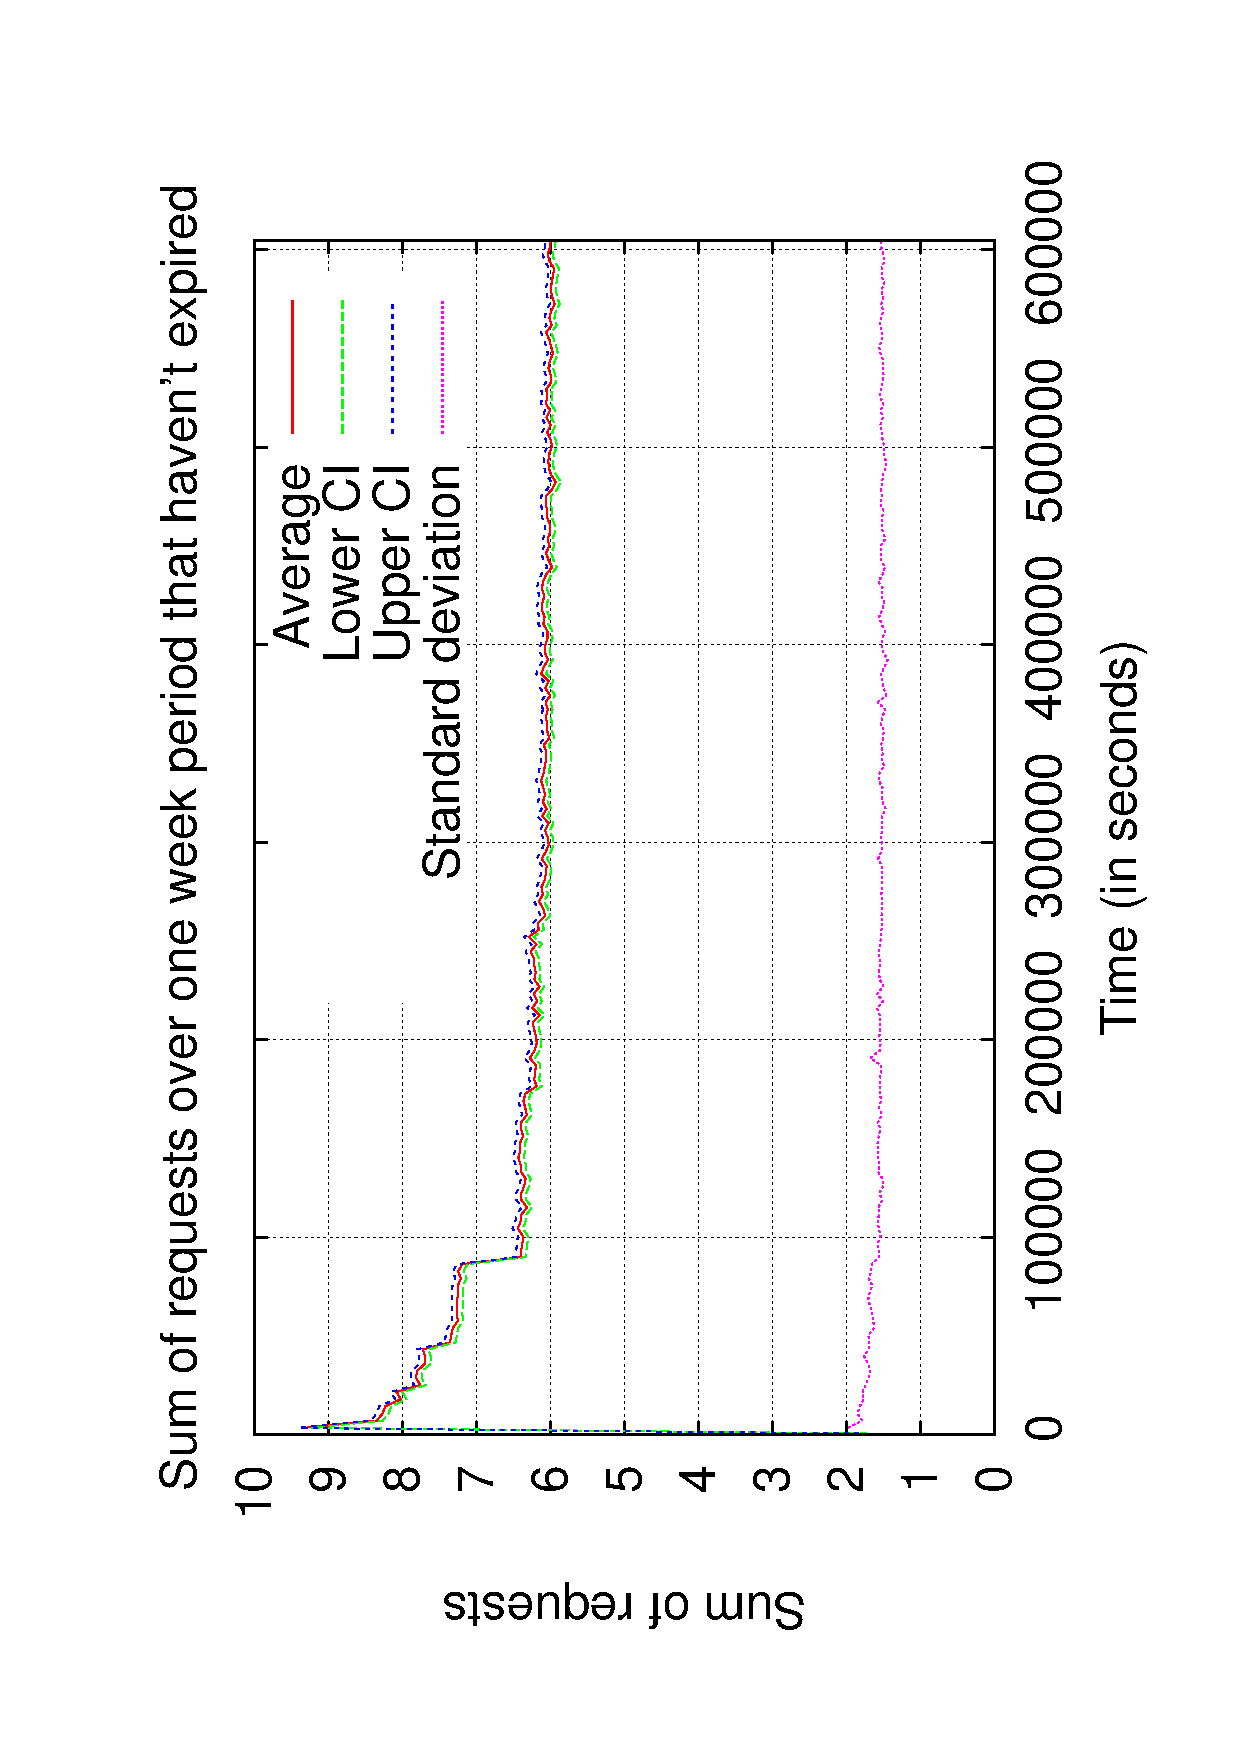
\includegraphics[width=.95\linewidth]{Sum_of_requests_over_time}
	\caption{Sum of requests over time  }
	\label{fig:sim_req}
\end{figure}

\begin{figure}
	\centering
	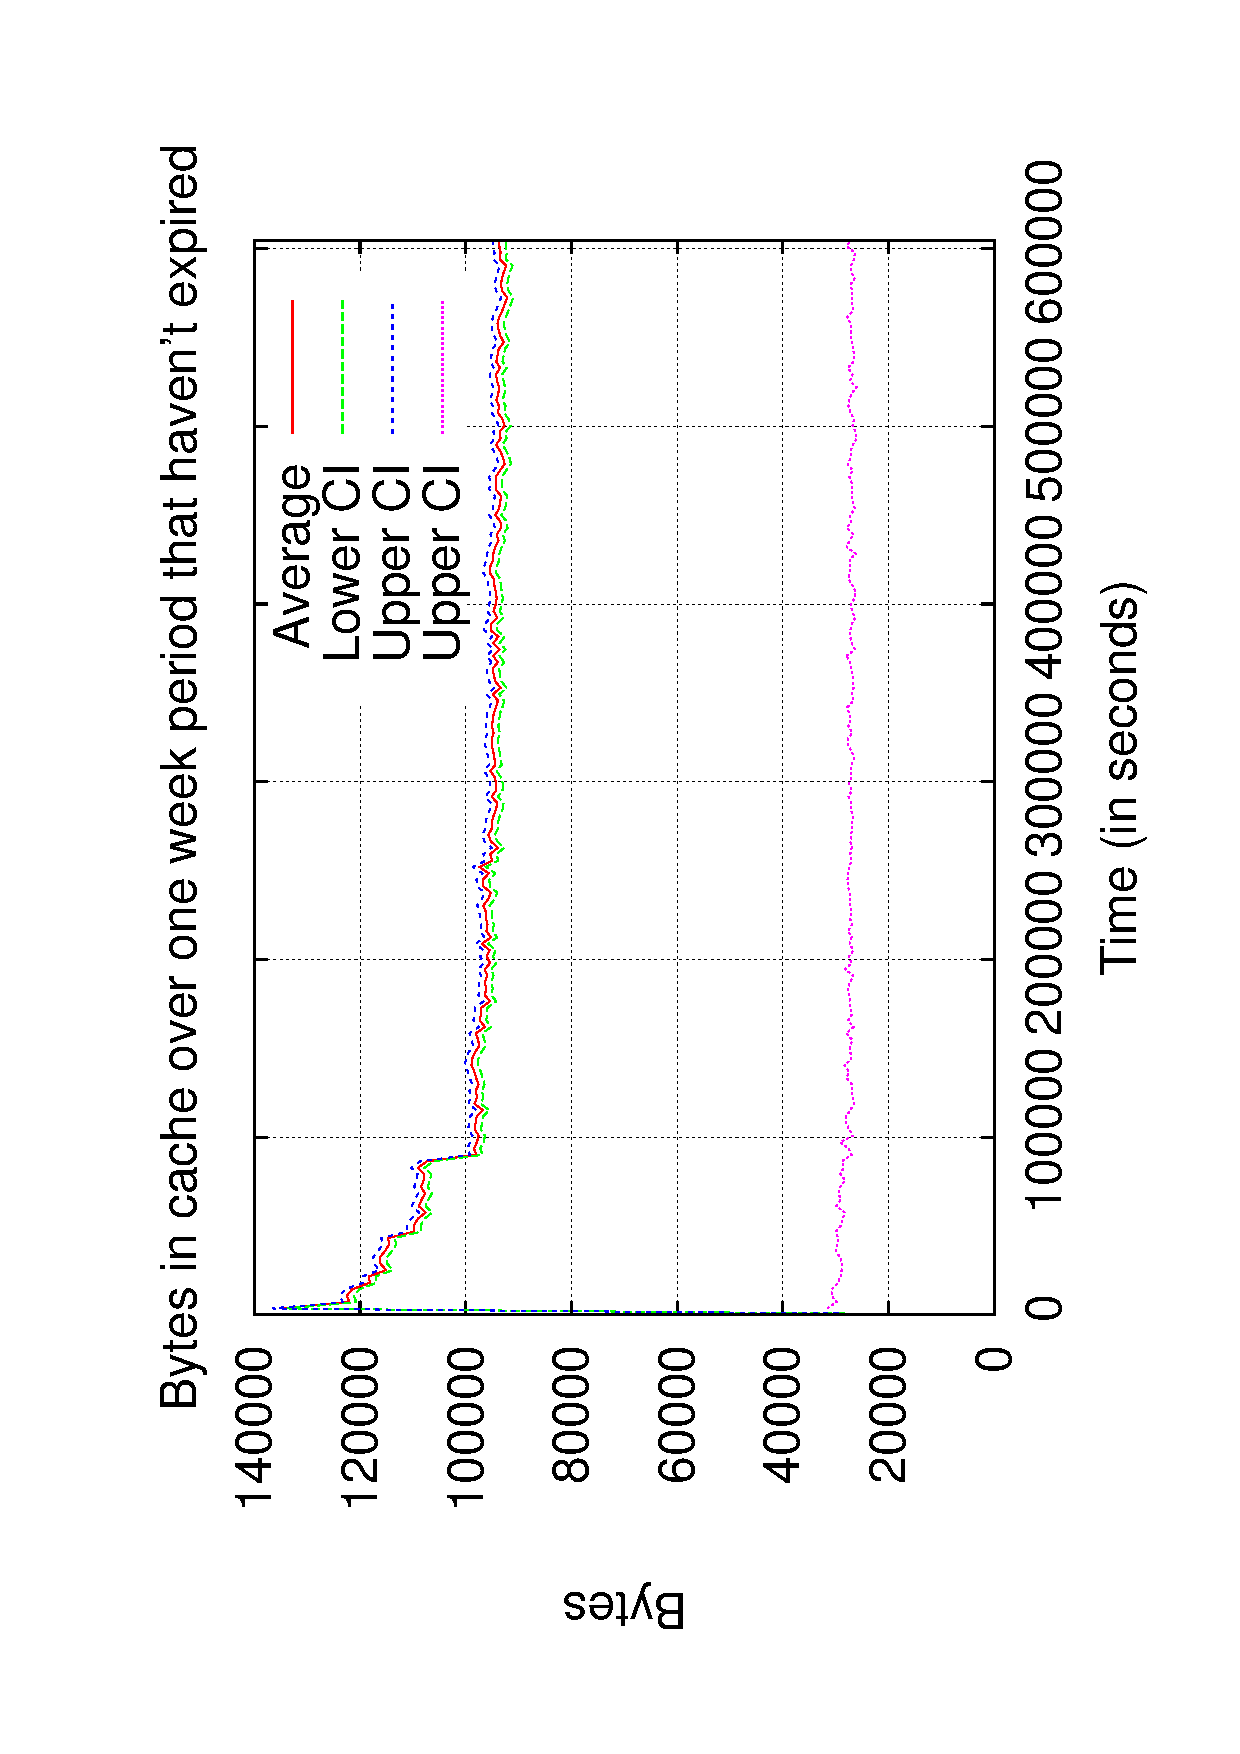
\includegraphics[width=.95\linewidth]{Sum_of_bytes_over_time}
	\caption{Sum of requests over time  }
	\label{fig:sim_bytes}
\end{figure}



\begin{figure}
	\centering
	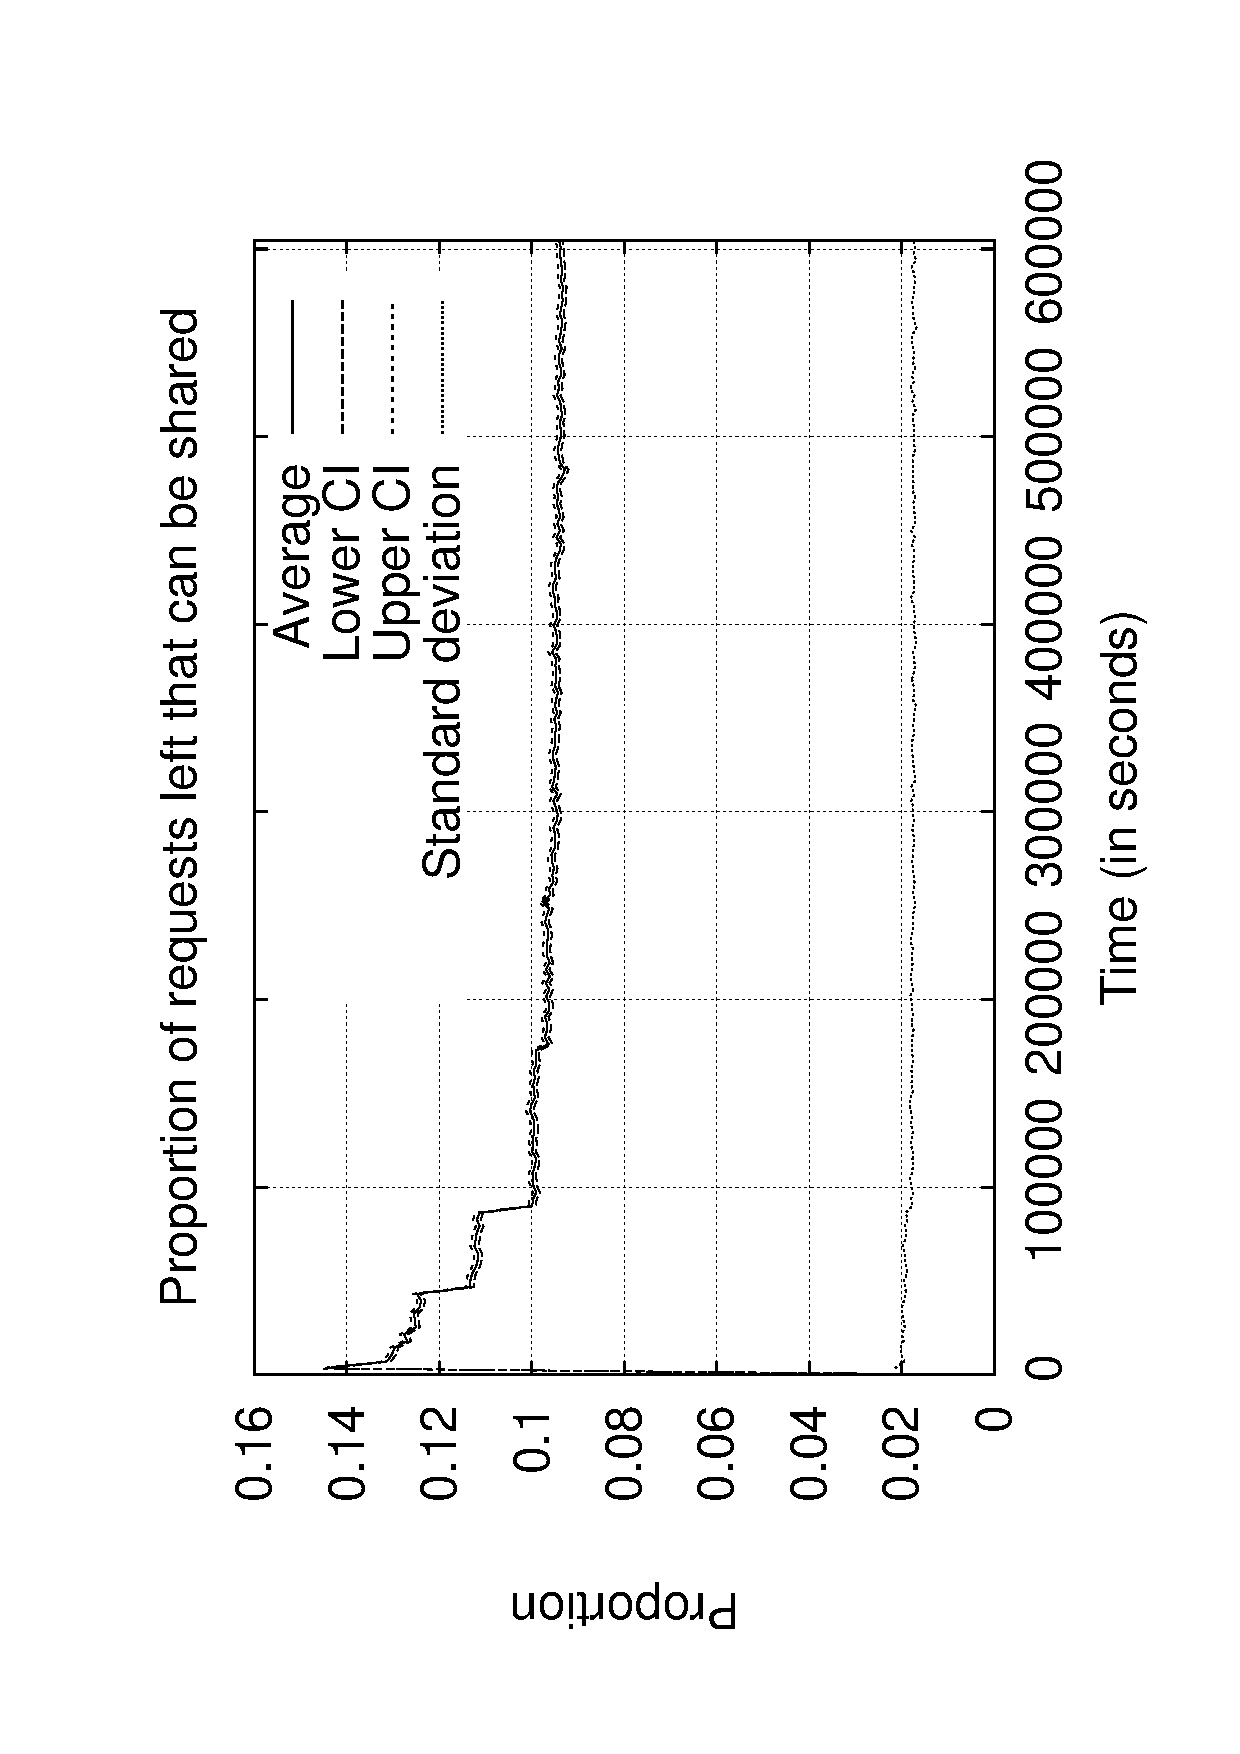
\includegraphics[width=.95\linewidth]{savings_Sum_of_requests_over_time}
	\caption{multiplied}
	\label{fig:sim_saver}
\end{figure}

\begin{figure}
	\centering
	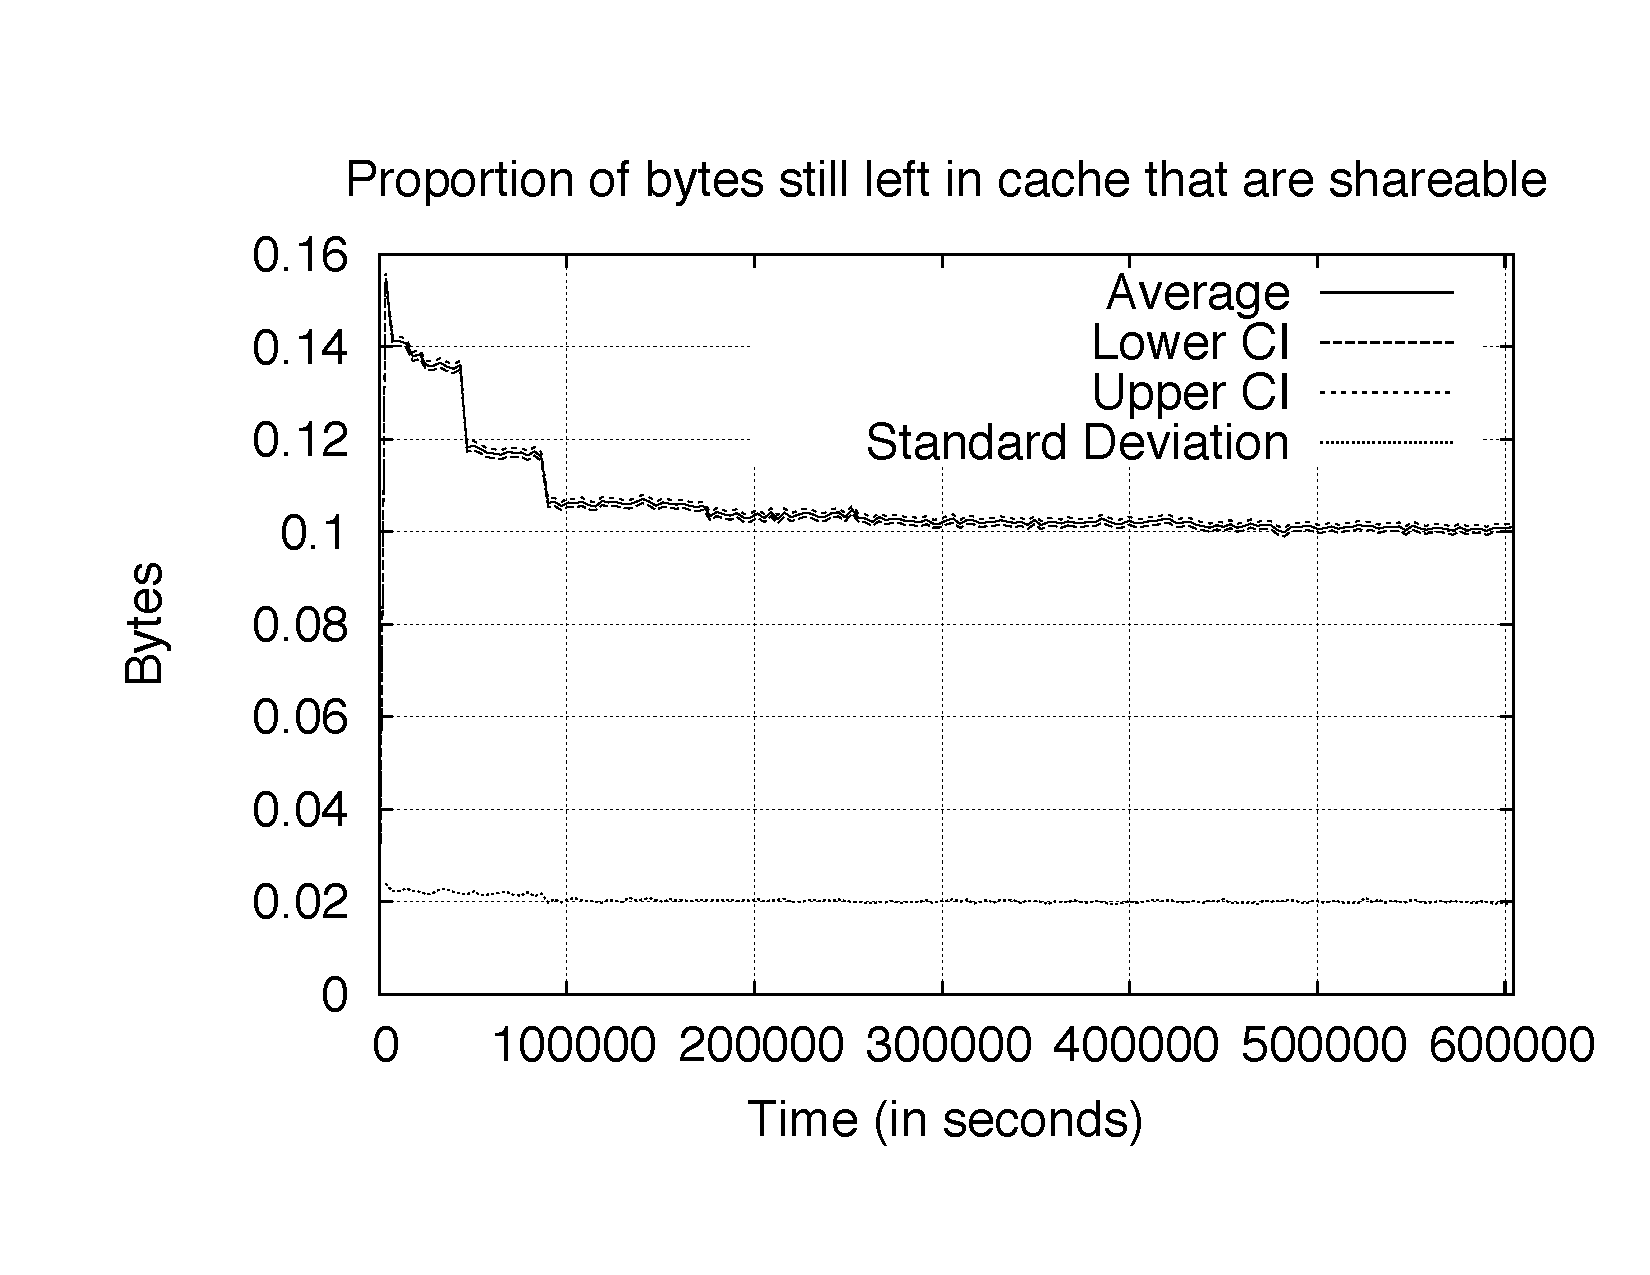
\includegraphics[width=.95\linewidth]{savings_Sum_of_bytes_over_time}
	\caption{multiplied}
	\label{fig:sim_saveb}
\end{figure}



\section{Conclusion}

\bibliographystyle{IEEEtran}
\bibliography{content}

\end{document}
